\documentclass[conference,letterpaper,10pt]{IEEEtran}
\usepackage{cite}
\usepackage{amsmath,amssymb}
\usepackage{booktabs}
\usepackage{url}
\usepackage{tikz}
\usetikzlibrary{arrows.meta,positioning}

\begin{document}

\title{Evidence-Aware Arrival-Time Parking Recommendations for New Taipei Roadside Parking}

\author{\IEEEauthorblockN{Changcun Liu}
\IEEEauthorblockA{National Chung Hsing University\\
Taichung, Taiwan}}

\maketitle

\begin{abstract}
Parking guidance is useful only if a reported space remains available when a driver arrives, not merely when a query is made. However, delayed or invalid observations, unsupported forecast horizons, and source failures can make arrival-time advice unreliable. To address this challenge, this paper proposes an evidence-aware agent for New Taipei roadside parking that validates source data, compares persistence, historical-median, and tree-model forecasts, ranks candidates by arrival-time fullness risk and distance, and uses bounded retries or abstention. Its development separates deterministic connectors and quality gates from validated prediction and planning, and prevents a language model from generating occupancy values. We specify, but do not claim to have completed, a chronological 60/20/20 evaluation with purged target boundaries for +30- and +60-minute horizons; metrics cover forecast error, calibrated full-occupancy risk, arrival-time Top-3 success, coverage, fault handling, and latency. Existing DIC3 project records report lower aggregate MAE for Persistence than for the two tree models, but these results are not independently reproduced and require boundary-corrected revalidation. No new recommendation gain, calibrated-risk gain, or agent superiority is claimed.
\end{abstract}

\begin{IEEEkeywords}
Smart parking, arrival-time prediction, AI agent, data quality, risk-aware recommendation, intelligent transportation systems.
\end{IEEEkeywords}

\section{Introduction}
\noindent\textbf{G. General.} Urban parking services increasingly use digital observations and prediction to help drivers locate spaces. Reviews of urban parking research describe a progression from statistical baselines to machine-learning and spatiotemporal methods \cite{ma2024}. For the driver, however, the operational target is not simply current occupancy: it is whether a candidate remains usable at the expected arrival time.

\noindent\textbf{H. However.} A vacancy shown at time $t$ may be occupied by $t+h$, where $h$ is the travel-to-arrival horizon. Delayed observations, missing fields, inconsistent capacity and failed sources can make a forecast misleading even when its model is accurate on clean data. SFpark reported weekday search time changing from 11 minutes 36 seconds to 6 minutes 36 seconds in pilot areas, while control areas changed by 13\% \cite{sfmta2014}. The pilot combined information, demand-responsive pricing and other measures; it motivates measuring search cost but is neither a New Taipei baseline nor evidence of this agent's effect. Research has also simulated how inaccurate on-street predictions can extend searching \cite{cao2025}.

\noindent\textbf{I. In literature.} Prior work includes surveys and simple forecasting baselines, spot-level duration models, graph-based curb and on-street predictors, cross-region learning, Bayesian uncertainty estimation and integrated parking decision support \cite{ma2024,schneble2025,cao2025,qian2025,vakrinou2026,kuang2025,nezhadettehad2025,piccialli2025}. These strands establish that prediction, uncertainty and integration are not individually new.

\noindent\textbf{J. Judgement.} The project-specific gap is narrower: whether source-quality gating, supported arrival-time risk and failure-aware orchestration improve roadside Top-$k$ decisions under matched constraints and inputs. A large model or an agent label alone does not establish that value. In the source-reported New Taipei aggregate comparison, Persistence has lower MAE than the tested tree models \cite{dic3design}, so the proposed evaluation must allow a simple baseline to remain the preferred model.

\noindent\textbf{K. Keypoint.} This paper makes three planned contributions: (1) an arrival-time recommendation contract that preserves per-candidate provenance and quality; (2) a constrained workflow with explicit retry, replan and abstention behavior; and (3) a falsifiable comparison of forecasts, rankings and orchestration against matched alternatives. H1 tests prediction error, H2 tests arrival-time Top-3 success, and H3 tests unsupported advice under injected failures. None is presumed to pass.

\noindent\textbf{L. Organization.} Section II positions related methods and summarizes their trade-offs. Section III defines the proposed agent, its data contract, ranking rule and operational example. Section IV specifies metrics, comparisons, setup, tuning and the limits of currently reported evidence. Section V concludes with the scope and outstanding tests.

\section{Related Work}
\noindent\textbf{M. Methods.} Simple persistence and historical summaries provide interpretable baselines for time-series prediction. Statistical occupancy-duration models address when individual spaces change state, while segment-level count forecasting uses a different target \cite{schneble2025}. Random forests and gradient-boosted trees model nonlinear temporal features; graph and multi-view neural methods add spatial relations, points of interest or external context for curb and on-street prediction \cite{cao2025,qian2025}. Multi-source garage studies and regional meta-learning broaden the data and transfer setting, but do not establish roadside performance in New Taipei \cite{vakrinou2026,kuang2025}.

Uncertainty-aware parking prediction is also established: Bayesian neural networks have been used to represent epistemic and aleatoric uncertainty \cite{nezhadettehad2025}. Integrated urban parking management and forecasting have been studied through digital-twin approaches \cite{piccialli2025}. These works make it inappropriate to claim that parking prediction has lacked uncertainty modeling or system integration. The UCI Birmingham dataset is useful for data-quality methods, but it contains off-street facility observations and cannot stand in for New Taipei curb ground truth \cite{stolfi2017}.

\noindent\textbf{N. New proposed.} The proposed distinction is an application-specific test of an evidence contract spanning source freshness, horizon support, candidate-level quality, calibrated risk and explicit failure handling. The system combines known components; its novelty claim is limited to evaluating whether that combination improves supported arrival-time curb recommendations over simpler methods using the same inputs. New Taipei prediction remains proposed, and the separately documented Taichung information agent has future prediction disabled.

\noindent\textbf{O. Organize (SWOT).} Table~\ref{tab:swot} compares four method families. The opportunities identify testable extensions; the threats identify failure modes that must be controlled rather than hidden by aggregate accuracy.

\begin{table*}[t]
\caption{SWOT comparison of parking prediction and decision-support approaches}
\label{tab:swot}
\centering
\scriptsize
\renewcommand{\arraystretch}{1.12}
\begin{tabular}{p{0.13\textwidth}p{0.18\textwidth}p{0.18\textwidth}p{0.18\textwidth}p{0.18\textwidth}}
\toprule
Approach & Strength & Weakness & Opportunity & Threat \\
\midrule
Persistence and historical statistics & Transparent, inexpensive, strong local reference & Misses abrupt changes and spatial effects & Add matched horizons and segment strata & Stale or irregular inputs can make a simple forecast invalid \\
Tree and spatiotemporal models & Capture nonlinear and spatial-temporal patterns & Need sufficient, reliable history and leakage control & Test contextual features and subgroup gains & Complexity may lose to Persistence or fail under domain shift \\
Uncertainty and transfer methods & Represent model uncertainty or exploit related regions & Calibration and transfer depend on labels and domain fit & Use selective prediction and calibrated risk & An uncalibrated score can be mistaken for a probability \\
Integrated systems and agents & Coordinate sources, constraints and recovery actions & Integration alone does not prove decision value & Compare evidence-aware orchestration with a fixed pipeline & Retries, stale sources or automation bias can increase harm \\
\bottomrule
\end{tabular}
\end{table*}

\section{Proposed Scheme}
\subsection{PA--PC: Aim, basis, and cure}
\noindent\textbf{PA. Aim.} Given a destination, requested arrival time, vehicle or parking preference and maximum walking distance, estimate availability for eligible New Taipei roadside segments and return a small, evidence-backed ranking. The target is availability at arrival, not a claim of a deployed predictive service.

\noindent\textbf{PB. Based on.} For segment $s$, let $C_s$ be capacity, $O_{s,t+h}$ occupied spaces at the target time, $t$ the latest admissible information cutoff and $h\in\{30,60\}$ minutes. The availability target is
\begin{equation}
Y_{s,t+h}=\max(0,C_s-O_{s,t+h}),\qquad Z_{s,t+h}=\mathbb{1}[Y_{s,t+h}=0].
\label{eq:target}
\end{equation}
Only information available by $t$ may enter features or model selection. An unavailable target is missing, not a zero-valued vacancy.

\noindent\textbf{PC. Cure.} Separate source validation from model inference. Invalid schema, impossible occupancy, stale input or unsupported horizon blocks that candidate from risk-based ranking. The planner may retry a recoverable source or select another valid source within a fixed budget. If no defensible evidence remains, it abstains or requests confirmation rather than converting unknown status to availability.

\subsection{PD--PG: Design, elements, and architecture}
\noindent\textbf{PD. Design.} The design moves the decision boundary from ``available now'' to ``supported at the requested arrival time.'' Each candidate carries its own source timestamp, validation state, forecast horizon and evidence; quality from one segment cannot be borrowed by another. This is a project design principle, not a claim that the field has never used predictive parking systems.

\noindent\textbf{PE. Paper elements.} The proposed components are a request parser, planner and tool registry, JSON/JSONL connectors, a schema/freshness/capacity gate, past-only feature generation, baseline or validated predictor, risk and domain rules, a Top-$k$ evidence response, and an arrival-verification record. The DIC3 design describes a separate Taichung current-information workflow and GIS implementation; it does not demonstrate a New Taipei prediction service \cite{dic3design}.

\noindent\textbf{PF. Foundation.} Define the candidate validity indicator
\begin{equation}
\begin{aligned}
V_s={}&\mathbb{1}[\text{schema valid}]\,\mathbb{1}[0\leq O_{s,t}\leq C_s]\\
&\mathbb{1}[0\leq t-t_s\leq\tau]\,\mathbb{1}[h\in\mathcal{H}].
\end{aligned}
\label{eq:valid}
\end{equation}
where $t_s$ is the observation time, $\tau>0$ a pre-registered freshness limit and $\mathcal{H}$ the validated horizon set. The freshness gate rejects future-dated observations. Let $D_s$ be estimated straight-line distance and $D_{\max}$ the walking constraint; candidates must satisfy $D_s\leq D_{\max}$. Define normalized distance as
\begin{equation}
\widetilde{D}_s=\begin{cases}
D_s/D_{\max}, & D_{\max}>0,\\
0, & D_{\max}=0\text{ and }D_s=0.
\end{cases}
\label{eq:distance}
\end{equation}
For valid candidates, let $p_s$ be a calibrated probability of full occupancy only when calibration and labels pass validation. Define the freshness score $Q_s=1-(t-t_s)/\tau$, which lies in $[0,1]$ under Eq.~(\ref{eq:valid}); schema and capacity remain hard gates, so this soft quality term measures observation recency only. A lower-is-better ranking score is
\begin{equation}
J_s=\lambda_d\widetilde{D}_s+\lambda_r p_s+\lambda_q(1-Q_s),\quad \lambda_d,\lambda_r,\lambda_q\geq 0.
\label{eq:rank}
\end{equation}
Weights and thresholds are selected on validation data. If calibrated $p_s$ is unavailable, the system must not label a raw score as probability or claim a validated risk-aware recommendation; it uses an explicitly named baseline or abstains.

\noindent\textbf{PG. Graph.} Fig.~\ref{fig:architecture} shows the planned control and evidence path. A failure branch returns to bounded replanning; exhausting the budget ends in abstention, not a fabricated candidate.

\begin{figure*}[t]
\centering
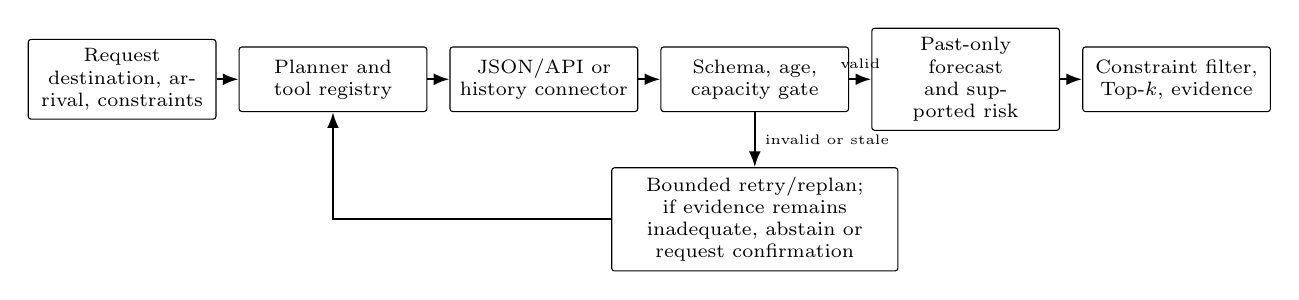
\begin{tikzpicture}[
  block/.style={draw,rounded corners=1pt,align=center,text width=2.15cm,minimum height=0.82cm,font=\scriptsize},
  flow/.style={-{Latex[length=2mm]},thick},
  node distance=0.28cm
]
\node[block] (request) {Request\\destination, arrival, constraints};
\node[block,right=of request] (planner) {Planner and\\tool registry};
\node[block,right=of planner] (source) {JSON/API or\\history connector};
\node[block,right=of source] (quality) {Schema, age,\\capacity gate};
\node[block,right=of quality] (model) {Past-only forecast\\and supported risk};
\node[block,right=of model] (rank) {Constraint filter,\\Top-$k$, evidence};
\node[block,below=0.7cm of quality,text width=3.4cm] (recover) {Bounded retry/replan; if evidence remains inadequate, abstain or request confirmation};
\draw[flow] (request) -- (planner);
\draw[flow] (planner) -- (source);
\draw[flow] (source) -- (quality);
\draw[flow] (quality) -- node[above,font=\tiny]{valid} (model);
\draw[flow] (model) -- (rank);
\draw[flow] (quality.south) -- node[right,font=\tiny]{invalid or stale} (recover.north);
\draw[flow] (recover.west) -| (planner.south);
\end{tikzpicture}
\caption{Proposed New Taipei arrival-time workflow. The figure is a design, not a deployment claim.}
\label{fig:architecture}
\end{figure*}

\subsection{PH--PI: Operation and interaction}
\noindent\textbf{PH. How.} The planner first normalizes the request and selects a connector with an applicable capability. Connectors return observations with source identity and timestamps. The quality gate checks required fields, capacity bounds, freshness and candidate identity. Valid records feed features derived only from the past. Prediction compares Persistence and same-weekday/time Historical Median with Random Forest and HistGradientBoosting. Risk calibration is a separate validation task. The ranking stage applies hard parking and distance constraints before sorting by Eq.~(\ref{eq:rank}).

\noindent\textbf{PI. Implementation and interaction.} The query path is: (1) parse destination, arrival time and limits; (2) select a source tool; (3) validate each candidate; (4) retry or replan only for recoverable failures and within a fixed budget; (5) forecast at a supported horizon; (6) rank feasible candidates and attach source time, model, limitations and evidence; and (7) record an arrival outcome only when a valid post-arrival observation exists. A fixed-pipeline comparator receives the same tools, data and retry budget. Haversine distance is an estimate, not routed walking distance. The language model may interpret and coordinate, but numerical occupancy and risk must come from validated tools.

\subsection{PJ--PM: Example, contributions, simulation, and property}
\noindent\textbf{PJ. Illustrative example.} Suppose candidate A is geographically closer but fails the pre-registered freshness gate, while candidate B is farther and passes schema, capacity and freshness checks. A is excluded from risk-based ranking; B may be returned with its evidence and estimated distance. If neither candidate passes, the response abstains. This hypothetical example explains the rule and is not a measured New Taipei observation.

\noindent\textbf{PK. Key contributions.} The contribution sought is (1) an explicit arrival-time target and per-candidate evidence contract, (2) a recoverable but bounded planner with an abstention state, and (3) a matched evaluation separating forecast, recommendation and orchestration effects. None implies that an agent is inherently superior to a fixed pipeline.

\noindent\textbf{PL. Simulation plan.} Section IV specifies chronological splits, matched horizons, baselines, outcome labels, fault cases and success criteria. The planned tests use the same test examples and operational constraints across comparators; they are not represented as completed simulations.

\noindent\textbf{PM. Mathematical property.} For a fixed valid candidate and nonnegative weights in Eq.~(\ref{eq:rank}), increasing normalized distance or calibrated fullness risk cannot improve its rank score, while increasing freshness cannot worsen it: $\partial J_s/\partial\widetilde{D}_s\geq0$, $\partial J_s/\partial p_s\geq0$, and $\partial J_s/\partial Q_s\leq0$. The validity and distance filters also ensure that an invalid or over-limit candidate is never ranked as eligible. These are properties of the proposed rule, not a proof of predictive accuracy or user benefit.

\section{Simulation}
\noindent\textbf{Q. Quality and quantity.} Forecast quality uses MAE and RMSE for available-space counts at +30 and +60 minutes. Full-occupancy risk uses PR-AUC, recall, Brier score and expected calibration error (ECE) only where labels and calibration are valid. Decision quality uses arrival-time Top-3 success, mean reciprocal rank, estimated distance, accepted-request coverage and abstention. Orchestration quality uses unsupported-recommendation rate, recovery outcome and 95th-percentile latency. Every metric reports its denominator, missing-label exclusions and time coverage.

\noindent\textbf{R. Related methods to compare.} H1 compares Persistence, same-weekday/time Historical Median, Random Forest and HistGradientBoosting on the same test rows. H2 compares risk-aware Top-3 with distance-only ranking at matched walking limits and accepted-request coverage. H3 compares the agent with a fixed pipeline under identical source access, models, timeout budget and injected timeout, stale-data and schema-error cases. The Birmingham off-street dataset may support quality-analysis tooling, but it is not a substitute for New Taipei roadside or arrival ground truth.

\noindent\textbf{S. Simulation setup.} The source design specifies New Taipei roadside JSONL, a global chronological 60/20/20 train/validation/test split, past-only features, matched test rows and exact +30/+60-minute targets \cite{dic3design}. Target timestamps crossing a split boundary must be purged; splitting feature rows alone is insufficient. Model selection and calibration use training/validation data, leaving the test set for final evaluation. Arrival outcomes require a pre-specified post-arrival tolerance window; absent valid observations remain missing. The data and full run are not included in this workspace, so the present paper cannot independently execute or reproduce that evaluation.

\noindent\textbf{T. Tuning.} Candidate lag and rolling windows, tree depth and leaf size, calibration method, freshness and capacity thresholds, ranking weights, retry limits and timeout budgets are selected using validation data only. The test set is not used to select features, thresholds or calibration. The final protocol records selected settings, software/data versions and the number of eligible examples for each horizon.

\noindent\textbf{U. Useful results currently available.} Table~\ref{tab:reported} transcribes the aggregate values reported in the project's DESIGN document \cite{dic3design}. They are source-reported and were not reproduced for this paper.

\begin{table}[t]
\caption{Source-reported New Taipei Phase 2 aggregate MAE}
\label{tab:reported}
\centering
\footnotesize
\begin{tabular}{lcc}
\toprule
Model & MAE (spaces) & Evidence status \\
\midrule
Persistence & 0.326757 & Reported; not reproduced \\
Random Forest & 0.402669 & Reported; not reproduced \\
HistGradientBoosting & 0.537539 & Reported; not reproduced \\
\bottomrule
\end{tabular}
\end{table}

The source reports 9,178,935 common test observations, with Persistence best in aggregate. It also notes 4,966 and 5,047 target timestamps crossing nominal split boundaries, a valid-observation grid rate of 54.26\%, and no-change proportions of 85.35\% at 30 minutes and 80.75\% at 60 minutes \cite{dic3design}. These figures require inspection of the full underlying report and corrected-purge reruns; they are not recalculated here. An earlier sample-notebook MAE near 7.12 spaces came from a different experiment and is not directly comparable. The reported aggregate does not support a claim that the tree models outperform Persistence.

\noindent\textbf{V. Verify effectiveness.} H1 passes only if the pre-registered model comparison improves on Persistence by the chosen threshold after boundary correction. H2 passes only with matched coverage and a pre-specified arrival label, alongside calibration and abstention results. H3 passes only if the agent reduces unsupported recommendations without concealing losses in coverage or unacceptable latency. The source design lists prospective gates including at least eight weeks of history, 90\% coverage, at least 5\% MAE improvement, full-occupancy recall of 0.80, a five-percentage-point Top-3 gain and p95 latency no greater than 3 s \cite{dic3design}. These are go/no-go targets, not achieved findings; their applicability must be fixed for the specific pilot and data contract before testing.

\section{Conclusion}
\noindent\textbf{W. What is proposed.} This paper specifies an evidence-aware agent for the gap between a parking query and arrival, where snapshot availability can become stale and source failures can invalidate otherwise plausible recommendations.

\noindent\textbf{X. Where it excels.} The design is specialized to constrained New Taipei roadside arrival-time decisions: it retains candidate-specific source evidence, uses simple baselines as credible comparators, and provides bounded recovery and abstention. It does not claim that these components are unprecedented across parking research.

\noindent\textbf{Y. Yields.} The only quantitative model comparison currently available is source-reported: Persistence has lower aggregate MAE than the two tree models. It is unreproduced here and has temporal-boundary and coverage limitations. No new simulation, arrival-time Top-3 benefit, calibrated-risk gain or agent-over-pipeline advantage is claimed.

\noindent\textbf{Z. Zen.} The next work is to acquire and version the permitted roadside history, purge boundary-crossing targets, rerun matched baselines, calibrate risk on held-out validation data, and evaluate arrival outcomes and injected failures. Deployment should follow only if these tests support useful, calibrated recommendations; otherwise the system should retain a transparent information-only or baseline workflow and abstain when evidence is inadequate.

\bibliographystyle{IEEEtran}
\bibliography{references,references_a2z}

\end{document}